\section{Результаты}

Описанная система уравнения персонажем была реализована на языке Python. Работа с кинематическим деревом реализована с помощью библиотеки pinocchio \cite{Carpentier}, \cite{Pinocchio}. Оптимизация выполняется с помощью библиотеки \cite{CVXOPT}. Данные библиотеки выбраны поскольку они реализуют необходимый функционал наиболее эффективным образом.

% NOTE: These values were selected experimentally
\begin{figure}
  \hfill
  \begin{minipage}{0.326\textwidth}
    \centering
    \includegraphics[scale=0.13]{animation/1.png}
  \end{minipage}
  \begin{minipage}{0.326\textwidth}
    \centering
    \includegraphics[scale=0.13]{animation/2.png}
  \end{minipage}
  \begin{minipage}{0.326\textwidth}
    \centering
    \includegraphics[scale=0.13]{animation/3.png}
  \end{minipage}
  \vfill
  \hfill
  \begin{minipage}{0.326\textwidth}
    \centering
    \includegraphics[scale=0.13]{animation/4.png}
  \end{minipage}
  \begin{minipage}{0.326\textwidth}
    \centering
    \includegraphics[scale=0.13]{animation/5.png}
  \end{minipage}
  \begin{minipage}{0.326\textwidth}
    \centering
    \includegraphics[scale=0.13]{animation/6.png}
  \end{minipage}
  \vfill
  \hfill
  \begin{minipage}{0.326\textwidth}
    \centering
    \includegraphics[scale=0.13]{animation/7.png}
  \end{minipage}
  \begin{minipage}{0.326\textwidth}
    \centering
    \includegraphics[scale=0.13]{animation/8.png}
  \end{minipage}
  \begin{minipage}{0.326\textwidth}
    \centering
    \includegraphics[scale=0.13]{animation/9.png}
  \end{minipage}
  \vfill
  \hfill
  \begin{minipage}{0.326\textwidth}
    \centering
    \includegraphics[scale=0.13]{animation/10.png}
  \end{minipage}
  \begin{minipage}{0.326\textwidth}
    \centering
    \includegraphics[scale=0.13]{animation/11.png}
  \end{minipage}
  \begin{minipage}{0.326\textwidth}
    \centering
    \includegraphics[scale=0.13]{animation/12.png}
  \end{minipage}
  \vfill
  \hfill
  \begin{minipage}{0.326\textwidth}
    \centering
    \includegraphics[scale=0.13]{animation/13.png}
  \end{minipage}
  \begin{minipage}{0.326\textwidth}
    \centering
    \includegraphics[scale=0.13]{animation/14.png}
  \end{minipage}
  \begin{minipage}{0.326\textwidth}
    \centering
    \includegraphics[scale=0.13]{animation/15.png}
  \end{minipage}
  \vfill
  \hfill
  \begin{minipage}{0.326\textwidth}
    \centering
    \includegraphics[scale=0.13]{animation/16.png}
  \end{minipage}
  \begin{minipage}{0.326\textwidth}
    \centering
    \includegraphics[scale=0.13]{animation/17.png}
  \end{minipage}
  \begin{minipage}{0.326\textwidth}
    \centering
    \includegraphics[scale=0.13]{animation/18.png}
  \end{minipage}
  \caption{Опорная анимация}
  \label{fig:reference}
\end{figure}

% NOTE: These values were selected experimentally
\begin{figure}
  \hfill
  \begin{minipage}{0.325\textwidth}
    \centering
    \includegraphics[scale=0.13]{balance/1.png}
  \end{minipage}
  \begin{minipage}{0.325\textwidth}
    \centering
    \includegraphics[scale=0.13]{balance/2.png}
  \end{minipage}
  \begin{minipage}{0.325\textwidth}
    \centering
    \includegraphics[scale=0.13]{balance/3.png}
  \end{minipage}
  \vfill
  \hfill
  \begin{minipage}{0.325\textwidth}
    \centering
    \includegraphics[scale=0.13]{balance/4.png}
  \end{minipage}
  \begin{minipage}{0.325\textwidth}
    \centering
    \includegraphics[scale=0.13]{balance/5.png}
  \end{minipage}
  \begin{minipage}{0.325\textwidth}
    \centering
    \includegraphics[scale=0.13]{balance/6.png}
  \end{minipage}
  \vfill
  \hfill
  \begin{minipage}{0.325\textwidth}
    \centering
    \includegraphics[scale=0.13]{balance/7.png}
  \end{minipage}
  \begin{minipage}{0.325\textwidth}
    \centering
    \includegraphics[scale=0.13]{balance/8.png}
  \end{minipage}
  \begin{minipage}{0.325\textwidth}
    \centering
    \includegraphics[scale=0.13]{balance/9.png}
  \end{minipage}
  \vfill
  \hfill
  \begin{minipage}{0.325\textwidth}
    \centering
    \includegraphics[scale=0.13]{balance/10.png}
  \end{minipage}
  \begin{minipage}{0.325\textwidth}
    \centering
    \includegraphics[scale=0.13]{balance/11.png}
  \end{minipage}
  \begin{minipage}{0.325\textwidth}
    \centering
    \includegraphics[scale=0.13]{balance/12.png}
  \end{minipage}
  \vfill
  \hfill
  \begin{minipage}{0.325\textwidth}
    \centering
    \includegraphics[scale=0.13]{balance/13.png}
  \end{minipage}
  \begin{minipage}{0.325\textwidth}
    \centering
    \includegraphics[scale=0.13]{balance/14.png}
  \end{minipage}
  \begin{minipage}{0.325\textwidth}
    \centering
    \includegraphics[scale=0.13]{balance/15.png}
  \end{minipage}
  \vfill
  \hfill
  \begin{minipage}{0.325\textwidth}
    \centering
    \includegraphics[scale=0.13]{balance/16.png}
  \end{minipage}
  \begin{minipage}{0.325\textwidth}
    \centering
    \includegraphics[scale=0.13]{balance/17.png}
  \end{minipage}
  \begin{minipage}{0.325\textwidth}
    \centering
    \includegraphics[scale=0.13]{balance/18.png}
  \end{minipage}
  \caption{Сбалансированная анимация наклона}
  \label{fig:result}
\end{figure}

Для демонстрации работы системы была разработана анимация наклона, кадры которой представлены на рисунке \ref{fig:reference}. Данная анимация не является сбалансированной, так как, например, проекция положения центр масс длительное время находится за пределами опорного полигона.

% Кадры движения, которое в результате работы разработанной системы, представлены на рисунке \ref{fig:result}. Основной цикл работы системы выполнялся 120 раз в секунду.

% Детальное отличие

% Панч про возможность настроить систему